\documentclass[a4paper,8pt]{beamer}
\usetheme{Madrid}
\usecolortheme{seahorse}
\usepackage[retainorgcmds]{IEEEtrantools}
\usepackage{graphicx}
\usepackage{physics}
\usepackage{bm,bbm}
\usepackage{tabularx,multirow,booktabs}
\usepackage{subcaption}
\usefonttheme{serif}
\title[Comm. analysis]{Research update}
\date{\today}
\author{Sree Ganesh}
\institute[U of A]{Schwartz Group \\ University of Arizona}
\begin{document}
\maketitle
%
%------------------------------------------------------------------------------
% SLIDE 1
%------------------------------------------------------------------------------
%
%\begin{frame}
%\frametitle{Contents}
%\begin{itemize}
%  \item Introduction
%	\item Convergence tests
%	\item Hartree-Fock and the case of Conjugated acenes
%	\item Sodium clusters and inclusion of temperature effects
 %  \item Non-orbital-optimized RPA based polarizabilities 
%\end{itemize}
%\end{frame}
%------------------------------------------------------------------------------
%
%------------------------------------------------------------------------------
% SLIDE 6
%------------------------------------------------------------------------------
%
\begin{frame}
\frametitle{MAT2A transition state}

\begin{figure}
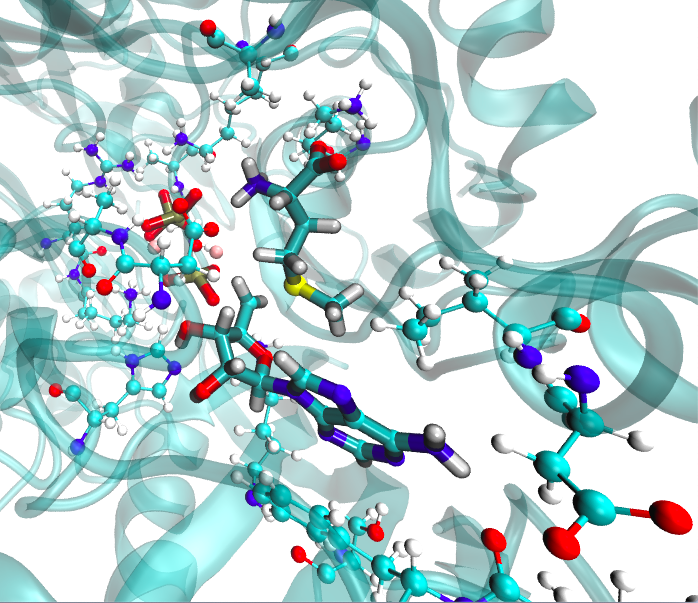
\includegraphics[scale=0.3]{ts_mat2a.png}
\end{figure}
\end{frame}

\begin{frame}
\frametitle{Commitor distributions for MAT2A}
\begin{figure}
\includegraphics[scale=0.33]{dist_1.pdf}
\end{figure}
\begin{figure}
\includegraphics[scale=0.33]{dist_2.pdf}
\end{figure}
\end{frame}
%



\end{document}
